\documentclass{article}
\usepackage[utf8]{inputenc}
\usepackage[margin=0.9in]{geometry}
\usepackage{graphicx}
\usepackage{indentfirst}
\usepackage{mathtools}
\newcommand{\horrule}[1]{\rule{\linewidth}{#1}}

\title{
	\normalfont\normalsize
    \textsc{McGill University}
    \horrule{0.5pt} \\[0.3cm]
	\huge Assignment 2
    \horrule{2pt} \\[0.3cm]
}

\author{
	Nabil Chowdhury \\
	\small{ID: 260622155} \\
    \small{COMP 551}
}

\date{\normalsize\today}

\begin{document}
\maketitle

% Question 1
\section{Generating DS1}
The code explains this step clearly. The data is shuffled and then output to DS1\_test and DS1\_train. The test set contains 1200 examples (600 positive, 600 negative), and the train set contains 2800 examples (1400 positive, 1400 negative).

% Question 2
\section{Probabilistic LDA Model}
Using the data generated in Question 1, the parameters of the probabilistic LDA model were found and used to calculate the coefficients \(w_0\) and \(\mathbf{w}\):\\

\[w_0 = -27.22691891296201\]
\begin{equation}
	\mathbf{w}=
	\begin{bmatrix}
		-14.35081404\\
        8.51556309\\
        5.75326526\\
        3.21580021\\
        9.56280808\\
        4.26881422\\
        -17.11861584\\
        23.83916969\\
        29.0419213\\
        -9.05879699\\
        13.18260588\\
        12.4169004\\
        -15.51799165\\
        -12.95808369\\
        5.72465615\\
        -12.90280764\\
        -29.42539436\\
        6.57706464\\
        0.6836093\\
        4.99936544
	\end{bmatrix}
\end{equation}

\newpage
These coefficients were used to obtain the following metrics from the test set:
\begin{center}
\begin{tabular}{ |c|c| }
	\hline
	\textbf{Metric} & \textbf{Score} \\
	\hline
	Accuracy & 0.9525 \\
	Precision & 0.95 \\
	Recall & 0.95477 \\
    F-Measure & 0.95238 \\
	\hline
\end{tabular}
\end{center}

% Question 3
\section{K Nearest Neighbors}
Odd k values from 1 to 99 inclusive were tested. KNN performs significantly worse than the linear model for all values of k tested. Here is a plot of K vs the four metrics:

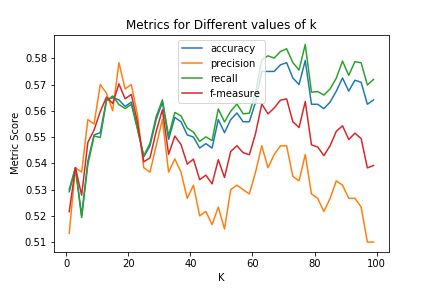
\includegraphics[width=\linewidth]{knn_q3.png}

The best k for accuracy and recall was 77. The best k for precision and F-score was 17. It is clear from the plot that certain values of K perform better than others, but all are much worse when compared to the linear model.

The raw scores for all k is shown below, with k=17 and k=77 rows bolded:
\begin{center}
\begin{tabular}{ |c|c|c|c|c| }
	\hline
	\textbf{K value} & \textbf{Accuracy} & \textbf{Precision} & \textbf{Recall} & \textbf{F-Measure}\\
	\hline
	1 &  0.52917 &  0.51333 &  0.53012 &  0.52159 \\
    3 &  0.53833 &  0.53833 &  0.53833 &  0.53833 \\
    5 &  0.52000 &  0.53667 &  0.51935 &  0.52787 \\
    7 &  0.54083 &  0.55667 &  0.53958 &  0.54799 \\
    9 &  0.55083 &  0.55500 &  0.55041 &  0.55270 \\
    11 &  0.55167 &  0.57000 &  0.54984 &  0.55974 \\
    13 &  0.56417 &  0.56667 &  0.56385 &  0.56525 \\
    15 &  0.56500 &  0.56000 &  0.56566 &  0.56281 \\
    \textbf{17} &  0.56417 &  \textbf{0.57833} &  0.56240 &  \textbf{0.57025} \\
    19 &  0.56167 &  0.56833 &  0.56086 &  0.56457 \\
    21 &  0.56333 &  0.57000 &  0.56250 &  0.56623 \\
    23 &  0.55333 &  0.55833 &  0.55281 &  0.55556 \\
    25 &  0.54250 &  0.53833 &  0.54286 &  0.54059 \\
    27 &  0.54667 &  0.53667 &  0.54762 &  0.54209 \\
    29 &  0.55667 &  0.54667 &  0.55782 &  0.55219 \\
    31 &  0.56333 &  0.55667 &  0.56419 &  0.56040 \\
    33 &  0.54917 &  0.53667 &  0.55043 &  0.54346 \\
    35 &  0.55750 &  0.54167 &  0.55938 &  0.55038 \\
    37 &  0.55583 &  0.53667 &  0.55806 &  0.54715 \\
    39 &  0.55083 &  0.52667 &  0.55342 &  0.53971 \\
    41 &  0.55000 &  0.53167 &  0.55190 &  0.54160 \\
    43 &  0.54583 &  0.52000 &  0.54833 &  0.53379 \\
    45 &  0.54750 &  0.52167 &  0.55009 &  0.53550 \\
    47 &  0.54583 &  0.51667 &  0.54867 &  0.53219 \\
    49 &  0.55667 &  0.52333 &  0.56071 &  0.54138 \\
    51 &  0.55167 &  0.51500 &  0.55576 &  0.53460 \\
    53 &  0.55667 &  0.53000 &  0.55986 &  0.54452 \\
    55 &  0.55917 &  0.53167 &  0.56261 &  0.54670 \\
    57 &  0.55583 &  0.53000 &  0.55888 &  0.54405 \\
    59 &  0.55583 &  0.52833 &  0.55908 &  0.54327 \\
    61 &  0.56333 &  0.53667 &  0.56690 &  0.55137 \\
    63 &  0.57500 &  0.54667 &  0.57951 &  0.56261 \\
    65 &  0.57500 &  0.53833 &  0.58094 &  0.55882 \\
    67 &  0.57500 &  0.54333 &  0.58007 &  0.56110 \\
    69 &  0.57750 &  0.54667 &  0.58259 &  0.56406 \\
    71 &  0.57833 &  0.54667 &  0.58363 &  0.56454 \\
    73 &  0.57250 &  0.53500 &  0.57838 &  0.55584 \\
    75 &  0.57000 &  0.53333 &  0.57554 &  0.55363 \\
    \textbf{77} &  \textbf{0.57917} &  0.54333 &  \textbf{0.58528} &  0.56353 \\
    79 &  0.56250 &  0.52833 &  0.56708 &  0.54702 \\
    81 &  0.56250 &  0.52667 &  0.56732 &  0.54624 \\
    83 &  0.56083 &  0.52167 &  0.56600 &  0.54293 \\
    85 &  0.56333 &  0.52667 &  0.56835 &  0.54671 \\
    87 &  0.56750 &  0.53333 &  0.57245 &  0.55220 \\
    89 &  0.57250 &  0.53167 &  0.57895 &  0.55430 \\
    91 &  0.56750 &  0.52667 &  0.57350 &  0.54909 \\
    93 &  0.57167 &  0.52667 &  0.57875 &  0.55148 \\
    95 &  0.57083 &  0.52333 &  0.57827 &  0.54943 \\
    97 &  0.56250 &  0.51000 &  0.56983 &  0.53826 \\
    99 &  0.56417 &  0.51000 &  0.57196 &  0.53921 \\
	\hline
\end{tabular}
\end{center}


% Question 4
\section{Generating DS2}
The code explains this step clearly. The data is shuffled and then output to DS2\_test and DS2\_train. The test set contains 1200 examples (600 positive, 600 negative), and the train set contains 2800 examples (1400 positive, 1400 negative).

% Question 5
\section{LDA and KNN on DS2}
\subsection{LDA}
Using the data generated in Question 4, the parameters of the probabilistic LDA model were found and used to calculate the coefficients \(w_0\) and \(\mathbf{w}\):\\

\[w_0 = 0.07921153907637934\]
\begin{equation}
	\mathbf{w}=
	\begin{bmatrix}
		 0.04124253 \\
        -0.00244305 \\
        -0.01366028 \\
         0.01470345 \\
        -0.03887653 \\
        -0.03692325 \\
         0.04821048 \\
         0.04070492 \\
        -0.03958812 \\
        -0.05941566 \\
        -0.11504490 \\
         0.03493932 \\
         0.08516702 \\
         0.00812546 \\
        -0.00383386 \\
        -0.08377713 \\
        -0.10174113 \\
        -0.02114581 \\
         0.10470002 \\
         0.06721695 \\
	\end{bmatrix}
\end{equation}

These coefficients were used to obtain the following metrics from the test set:
\begin{center}
\begin{tabular}{ |c|c| }
	\hline
	\textbf{Metric} & \textbf{Score} \\
	\hline
	Accuracy & 0.51666 \\
	Precision & 0.51 \\
	Recall & 0.51689 \\
    F-Measure & 0.51342 \\
	\hline
\end{tabular}
\end{center}

We notice that when the data is generate by multiple Gaussian distributions, the performance of LDA takes a major hit. Let's look at KNN's performance before further comparison.

\subsection{KNN}
Here is a plot of K vs the four metrics: \\
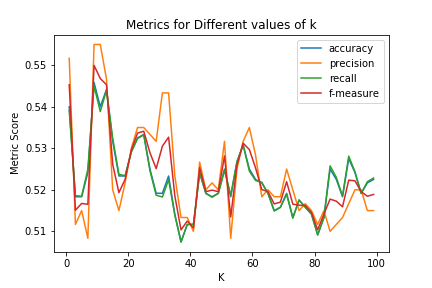
\includegraphics[width=\linewidth]{knn_q5.png}

The optimal K value was 47 for all four metrics. The full performance metric for all Ks tested is shown below:

\begin{center}
\begin{tabular}{ |c|c|c|c|c| }
	\hline
	\textbf{K value} & \textbf{Accuracy} & \textbf{Precision} & \textbf{Recall} & \textbf{F-Measure}\\
	\hline
	1 &  0.50500 &  0.51000 &  0.50495 &  0.50746 \\
    3 &  0.52833 &  0.53833 &  0.52778 &  0.53300 \\
    5 &  0.51167 &  0.52500 &  0.51136 &  0.51809 \\
    7 &  0.52833 &  0.54500 &  0.52742 &  0.53607 \\
    9 &  0.53250 &  0.54000 &  0.53202 &  0.53598 \\
    11 &  0.51917 &  0.52333 &  0.51901 &  0.52116 \\
    13 &  0.51583 &  0.52667 &  0.51550 &  0.52102 \\
    15 &  0.52333 &  0.53833 &  0.52265 &  0.53038 \\
    17 &  0.52417 &  0.53667 &  0.52358 &  0.53004 \\
    19 &  0.51917 &  0.54167 &  0.51834 &  0.52975 \\
    21 &  0.51917 &  0.54333 &  0.51828 &  0.53051 \\
    23 &  0.52833 &  0.55500 &  0.52690 &  0.54058 \\
    25 &  0.52833 &  0.56333 &  0.52648 &  0.54428 \\
    27 &  0.52917 &  0.56833 &  0.52705 &  0.54691 \\
    29 &  0.52667 &  0.55500 &  0.52524 &  0.53971 \\
    31 &  0.53500 &  0.55667 &  0.53355 &  0.54486 \\
    33 &  0.53417 &  0.55833 &  0.53259 &  0.54516 \\
    35 &  0.53750 &  0.56833 &  0.53532 &  0.55133 \\
    37 &  0.54417 &  0.57667 &  0.54147 &  0.55851 \\
    39 &  0.54833 &  0.57667 &  0.54574 &  0.56078 \\
    41 &  0.53917 &  0.57333 &  0.53666 &  0.55439 \\
    43 &  0.55333 &  0.59000 &  0.54969 &  0.56913 \\
    45 &  0.55750 &  0.59333 &  0.55365 &  0.57281 \\
    \textbf{47} &  \textbf{0.56000} &  \textbf{0.60500} &  \textbf{0.55505} &  \textbf{0.57895} \\
    49 &  0.55250 &  0.60167 &  0.54780 &  0.57347 \\
    51 &  0.54750 &  0.59667 &  0.54325 &  0.56871 \\
    53 &  0.54917 &  0.60167 &  0.54449 &  0.57165 \\
    55 &  0.54083 &  0.58500 &  0.53752 &  0.56026 \\
    57 &  0.54083 &  0.58833 &  0.53729 &  0.56165 \\
    59 &  0.53000 &  0.59000 &  0.52679 &  0.55660 \\
    61 &  0.53250 &  0.59000 &  0.52915 &  0.55792 \\
    63 &  0.53750 &  0.59500 &  0.53363 &  0.56265 \\
    65 &  0.54083 &  0.59500 &  0.53684 &  0.56443 \\
    67 &  0.53417 &  0.58667 &  0.53092 &  0.55740 \\
    69 &  0.52667 &  0.57500 &  0.52432 &  0.54849 \\
    71 &  0.54167 &  0.58500 &  0.53834 &  0.56070 \\
    73 &  0.53417 &  0.57500 &  0.53159 &  0.55244 \\
    75 &  0.53500 &  0.57667 &  0.53231 &  0.55360 \\
    77 &  0.52583 &  0.57833 &  0.52338 &  0.54949 \\
    79 &  0.52417 &  0.56667 &  0.52227 &  0.54357 \\
    81 &  0.51917 &  0.55833 &  0.51777 &  0.53729 \\
    83 &  0.51833 &  0.56500 &  0.51677 &  0.53981 \\
    85 &  0.51583 &  0.57000 &  0.51429 &  0.54071 \\
    87 &  0.51583 &  0.55833 &  0.51459 &  0.53557 \\
    89 &  0.52083 &  0.57167 &  0.51891 &  0.54401 \\
    91 &  0.51333 &  0.56000 &  0.51220 &  0.53503 \\
    93 &  0.51750 &  0.56667 &  0.51593 &  0.54011 \\
    95 &  0.51667 &  0.56833 &  0.51511 &  0.54041 \\
    97 &  0.51750 &  0.56167 &  0.51608 &  0.53791 \\
    99 &  0.51583 &  0.56667 &  0.51437 &  0.53925 \\
	\hline
\end{tabular}
\end{center}

% Question 6
\section{Comparing performance of LDA and KNN on DS1 and DS2}

We can see that KNN actually beats LDA for DS2 (only slightly)! In fact, the performances of LDA and KNN for DS2 are quite similar to each other. When comparing the results to those of DS1, We see that KNN performs similarly for DS2, whereas LDA performs much worse for DS2 than DS1. This experiment provides evidence that KNN is less affected when the dataset is generated from a mixture of Gaussian distribution. LDA performs worse because the in-class variances are bigger for DS2 as compared to DS1 due to multiple different Gaussian distributions being used instead of just one.

\begin{thebibliography}{9}
\bibitem{All}
The following stackoverflow post was used to help in Q4 when dealing with multiple gaussians: https://stackoverflow.com/questions/39677967/python-sampling-from-different-distributions-with-different-probability
\end{thebibliography}

\end{document}
